\section{Preliminaries}

A graph $G=(V,E)$ consists of two components: a set of vertices or nodes $V$, and a set of edges $E \subseteq V \times V$. Generally, graphs can be categorized as being either directed or undirected based on their edge set $E$. A graph is undirected if and only if for any two nodes $u,v \in V$, $(u,v) \in E$ also implies $(v,u) \in E$ (and both correspond to the same undirected edge). In this paper, we restrict attention to undirected graphs.
%For citation networks, $v \rightarrow u \in E$ means paper $v$ cites paper $u$.

Let $|V|=n$ be the number of nodes and $m = |E|$ be the number of edges in $G$. Then, the graph adjacency matrix is the $n \times n$ matrix $\mathbf{A}$ with entries 
$$\mathbf{A}[i,j] =
\begin{cases}
    1 & \text{if } (i,j) \in E \\
    0 & \text{otherwise.}
\end{cases}$$ 
%The degree of a node $v$ is defined as $\text{deg}(v) = \sum_{j=1}^{n}\mathbf{A}[v,j]$, which is the number of papers cited by $v$ in the context of citation graphs. The degree of nodes naturally leads to the definition of the degree matrix of $G$: a degree matrix $\mathbf{D}$ is a $n\times n$ diagonal matrix with $\mathbf{D}[i,i] = \text{deg}(i)$. 
The Laplacian matrix or graph Laplacian is defined as $\mathbf{L} = \mathbf{D} - \mathbf{A}$, where $\bbD=\mbox{diag}(\bbA\boldsymbol{1})$ is the so-called degree matrix. From their definitions, and since $G$ is undirected, we can easily infer that $\mathbf{A}$ and $\bbL$ are symmetric.

%Prior works\cite{narang2011downsampling}\cite{geng2023pyramid} involving downsampling usually explores the spectral information of the Laplacian. 
In practice, real-world graphs are associated with node data $x \in \reals^n$ called graph signals, where $x[i]$ corresponds to the value of the signal at node $i$. More generally, graph signals consist of multiple features, in which case they are represented as matrices $X \in \mathbb{R}^{n \times d}$ with $d$ denoting the number of features. 
%As a result, the graph is constructed as a triplet $G(V,E,X)$.

The graph Laplacian plays an important role in graph signal processing (GSP) \cite{shuman13-mag,sandryhaila13-dspg}, as it allows defining the notion of total variation of a signal $x$. Explicitly, the total variation of $x$ is defined as $TV(x)=x^T\bbL x$ \cite{ortega2018graph}. Let $\bbL=\bbV\bbLam\bbV^T$ be the Laplacian eigendecomposition, where $\bbLam$ is a diagonal matrix with eigenvalues ordered as $\lambda_1 \leq \ldots \leq \lambda_n$ and $\bbV$ is the corresponding eigenvector matrix. For unit-norm signals, it is easy to see that the maximum total variation is $\lambda_n$, the largest Laplacian eigenvalue, and the minimum total variation is $\lambda_1=0$, which corresponds to the all-ones eigenvector. Therefore, the Laplacian eigenvalues can be interpreted as graph frequencies, and the eigenvectors as these frequencies' respective oscillation modes.

\subsection{Graph Neural Networks}

GNNs are a class of deep learning models specifically designed for graph-structured data. GNNs are layered architectures where each layer consists of two components: a bank of convolutional filters and a nonlinear activation function. 

A graph convolutional filter is the extension of a standard convolutional filter to graph data. More specifically, it consists of a shift-and-sum operation of a signal $x$ on the graph $G$. The notion of graph shift is captured by a matrix $\bbS \in \reals^{n\times n}$ encoding the sparsity pattern of the graph, i.e., $\bbS[i,j] \neq 0$ if and only if $(i,j) \in E$ or $i=j$; typical choices are $\bbS=\bbA$ or $\bbS=\bbL$ \cite{segarra17-linear}. The graph shift operator operates on $x$ as $\bbS x$.

Given any choice of $\bbS$, the graph convolution is defined as $y = \sum_{k=0}^{K-1} h_k \bbS^k x$, where $h_0, \ldots, h_{K-1}$ are the filter coefficients or taps. More generally, for $X \in \reals^{n \times d}$ and $Y \in \reals^{n\times f}$ we can define the convolutional filterbank \cite{gama18-gnnarchit}
\begin{equation}
     Y = \sum_{k=0}^{K-1} \bbS^k X \bbH_k
\end{equation}
where $\bbH_k \in \reals^{d \times f}$, $0 \leq k \leq K-1$, map $d$ features into $f$ features.

Equipped with the definition of graph convolution, we write the $\ell$th layer of a GNN as \cite{gama18-gnnarchit}
\begin{equation}
    X_{\ell} = \sigma \bigg( \sum_{k=0}^{K-1} \bbS^k X_{\ell-1} \bbH_{\ell k}\bigg)
\end{equation}
where $\sigma: \reals \to \reals$ is a pointwise nonlinearity (e.g., the ReLU or sigmoid) acting nodewise on the graph. At layer $\ell=1$, $X_0$ is the input data $X$, and the last layer output $X_L$ is the output $Y$ of the GNN. For succinctness, in the following we will represent the whole $L$-layer GNN as a map $Y = \Phi(X,G;\ccalH)$ with $\ccalH=\{\bbH_{\ell k}\}_{\ell,k}$.

% GNNs iteratively update node representations by aggregating information of the neighbors, enabling them to capture both local and global graph structure. This makes it preferable in dealing with relation datasets like social relations and citation networks. 

\noindent \textbf{Transferability.} The mathematical property that allows training GNNs on small graph subsamples of larger graphs is their transferability. Explicitly, GNNs are transferable in the sense that when a GNN with fixed weights $\ccalH$ is transferred across two graphs in the same ``family'', the transference error is upper bounded by a term that decreases with the graph size. Typical transferability analyses show this by defining graph ``families'' as graphs coming from the same random graph model, or converging to a common graph limit. Here, we consider families of graphs identified by the same graphon, which can be seen as both a generative model and a limit model for large graphs. 

A graphon is a bounded, symmetric, measurable function $\bbW: [0,1]^2 \to [0,1]$ \cite{borgs2008convergent,lovasz2012large}. Graphs can be sampled from $\bbW$ by sampling nodes $u_1, \ldots, u_n$ from $[0,1]$, and sampling edges $(u_i,u_j)$ with probability $\bbW(u_i,u_j)$. The graph limit interpretation is more nuanced but has to do with the fact that, on sequences of graphs converging to $\bbW$, the densities of certain ``motifs'', e.g., triangles, also converge. For graphs associated with the same graphon, we have the following transferability theorem.

% GNNs have shown promising results in various applications, including node classification, link prediction, and graph classification. However, the rapidly growing sizes of graphs pose a major concern to efficient training on GNNs. It is believed and shown that trained with subgraphs preserving the structural information, GNNs generalize well to the original full-size graphs\cite{ruiz2021graph}. Graph node downsampling can be seen as a special case of transferability\cite{ruiz2021graph} of GNNs where two graphs coming from the same graphon family have a closer relation. Namely, the smaller graph is the sampled subgraph of the bigger one. In addition, unlike other neural networks like MLP, GNN is more "independent" to the data/graph in the sense that it adapts to different input dimensions and graph structures. These desired properties imply the possibility of applying GNN trained over small subgraphs on huge but related graphs without changing the parameters. As a matter of fact, we have the following transferability theorem\cite{ruiz2021graph}

\begin{theorem}[GNN transferability, simplified \cite{ruiz2021transferability}]
    Let $\Phi$ be a GNN with fixed coefficients, and $G_n$, $G_m$ graphs with $n$ and $m$ nodes sampled from a graphon $\mathbf{W}$. Under mild conditions, $\| {\Phi}(G_n) - {\Phi}(G_m) \|= \mathcal{O}(n^{-1} + m^{-1})$ w.h.p..
\end{theorem}

In this paper, we will use the transferability property of GNNs, together with a novel graph sampling algorithm, to train GNNs on small graph subsamples and ensure they scale well to large graphs.

\begin{figure*}[t]
\centering
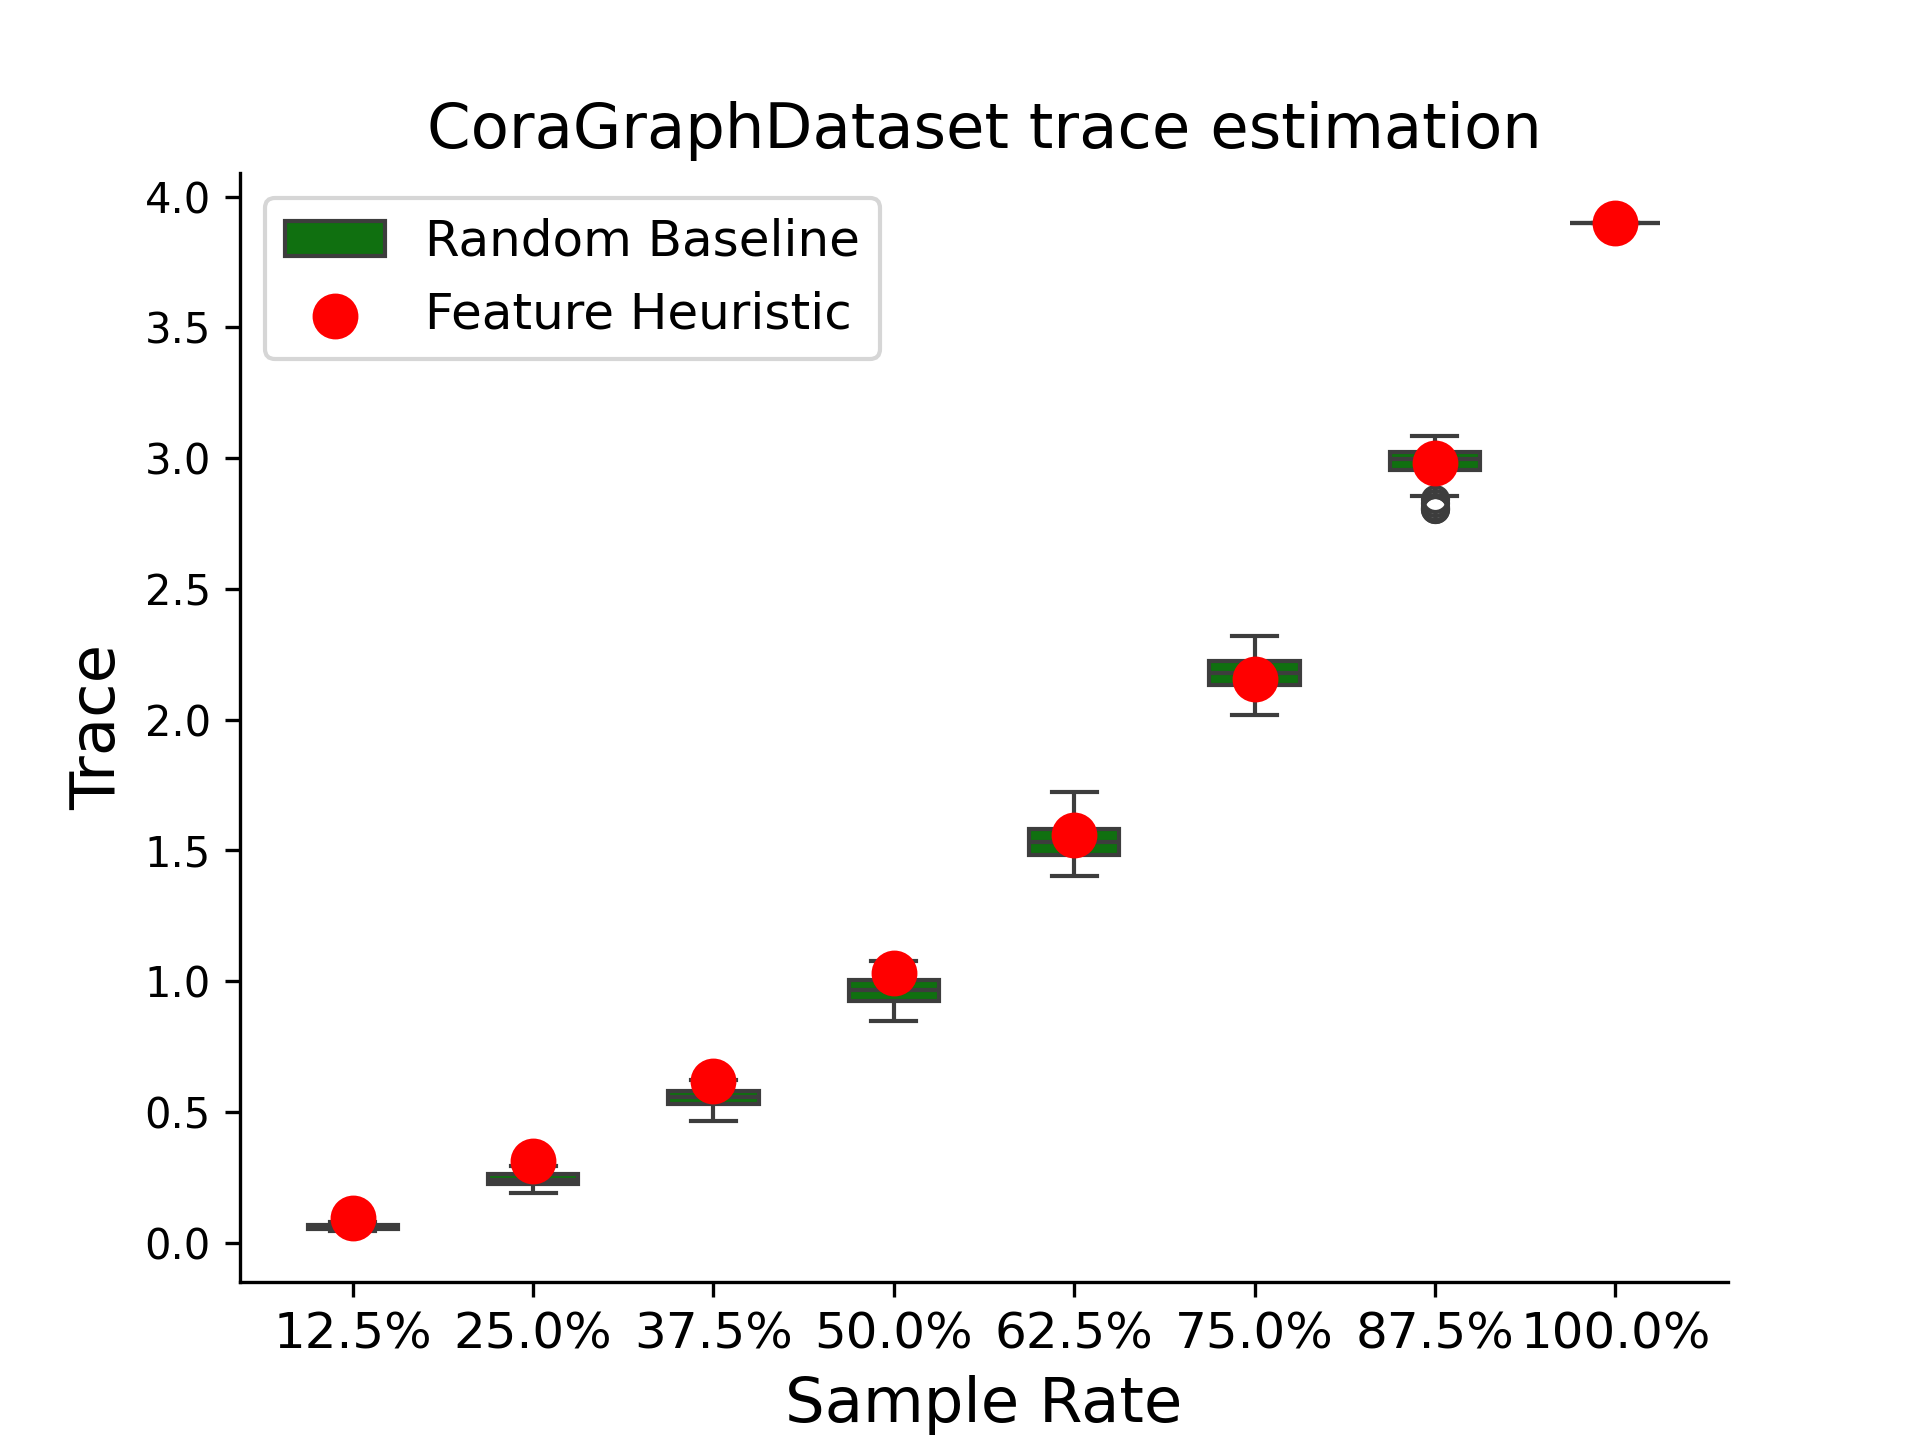
\includegraphics[width=0.32\textwidth]{img/trace_revised/CoraGraphDataset_trace_boxplot.png}
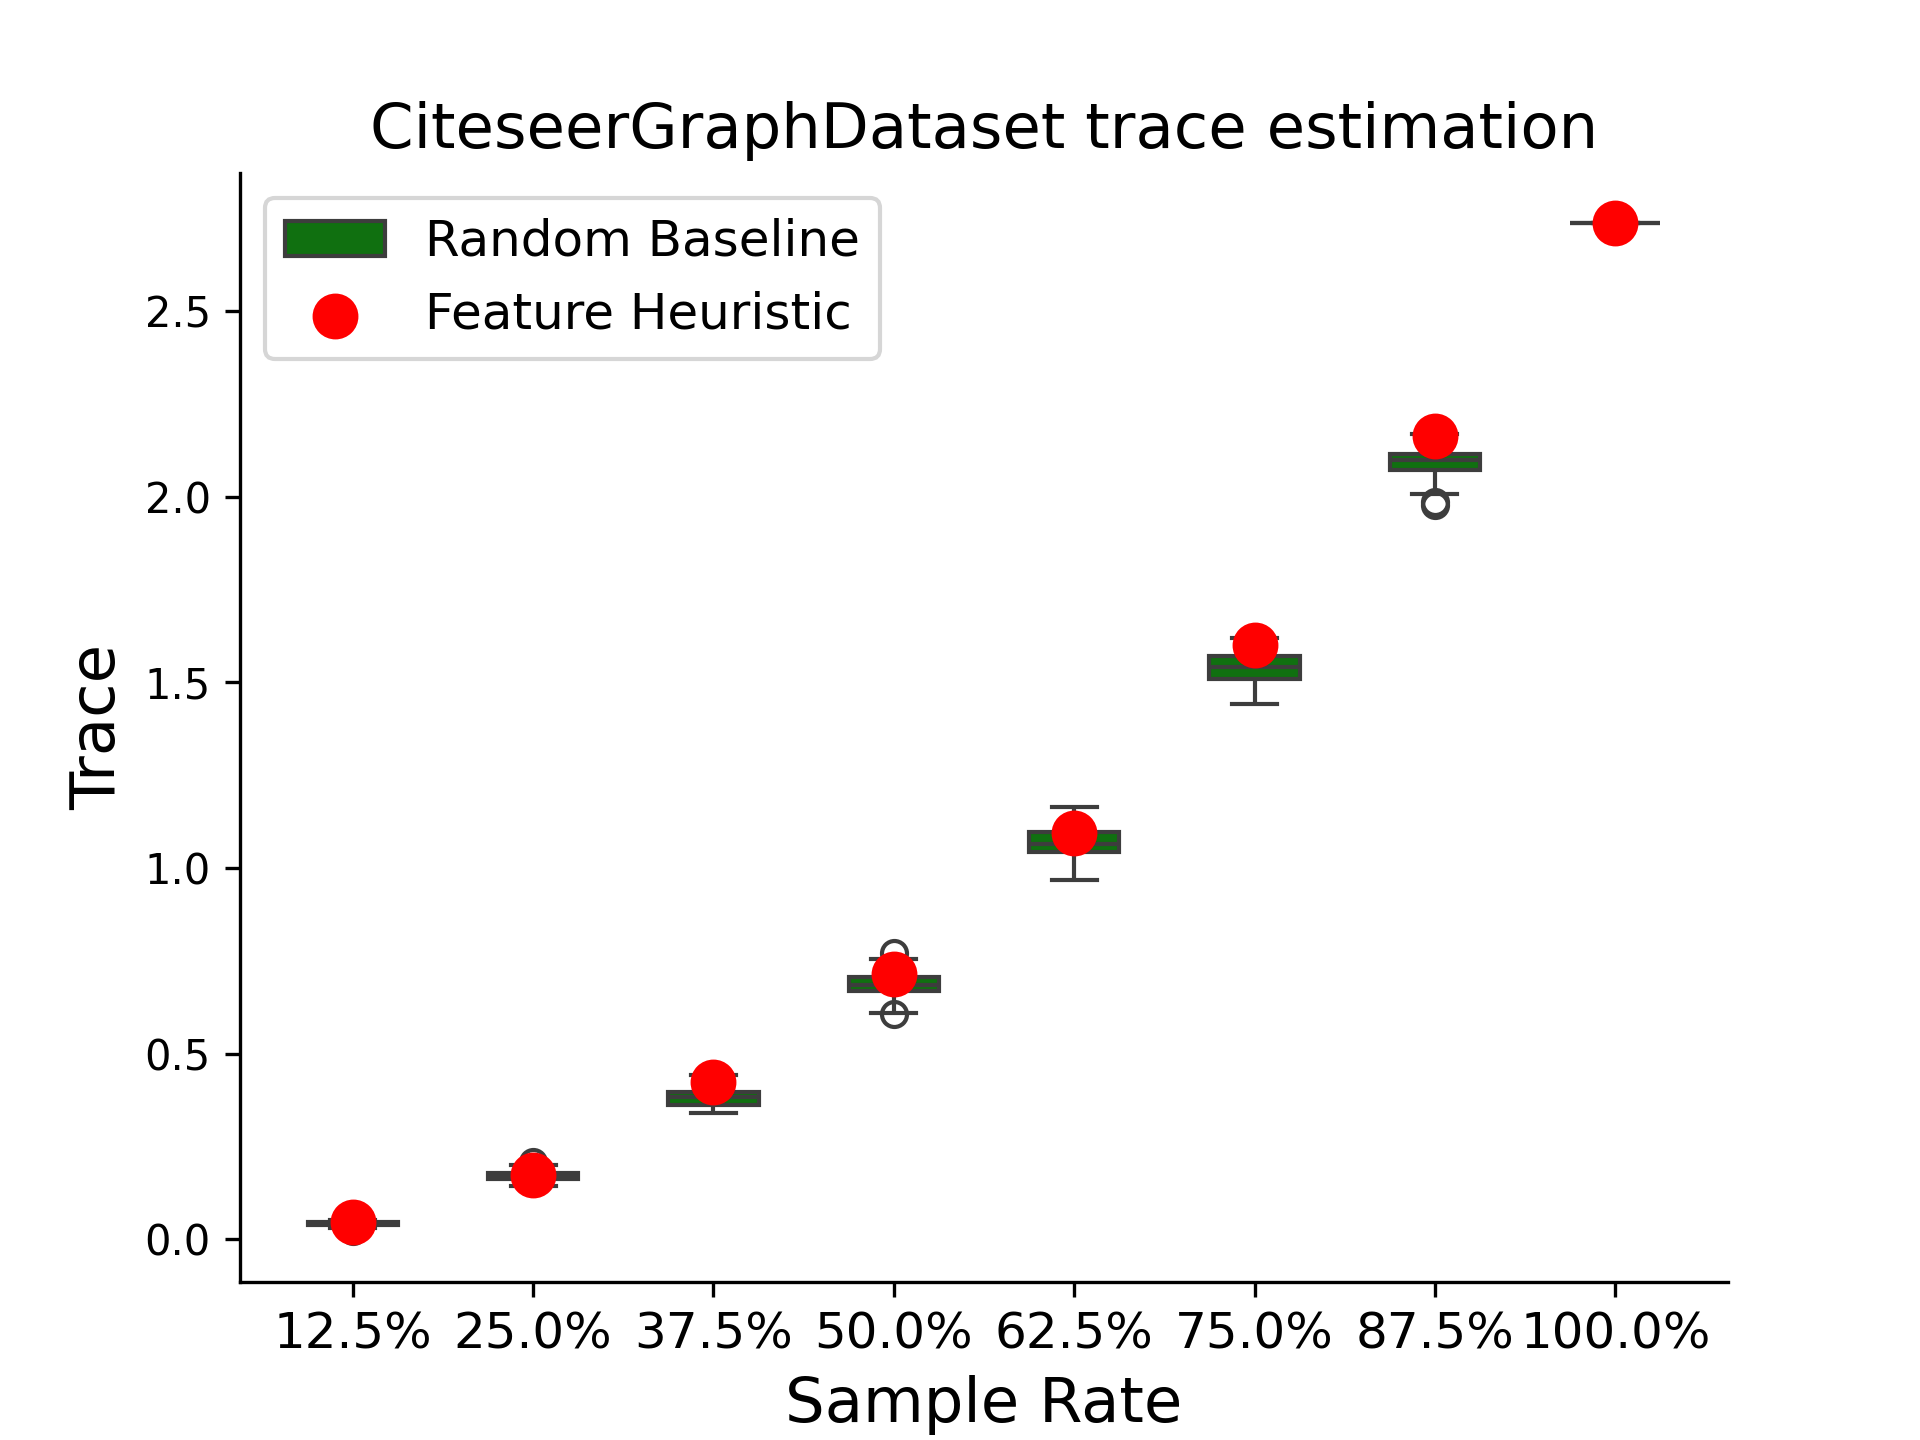
\includegraphics[width=0.32\textwidth]{img/trace_revised/CiteseerGraphDataset_trace_boxplot.png}
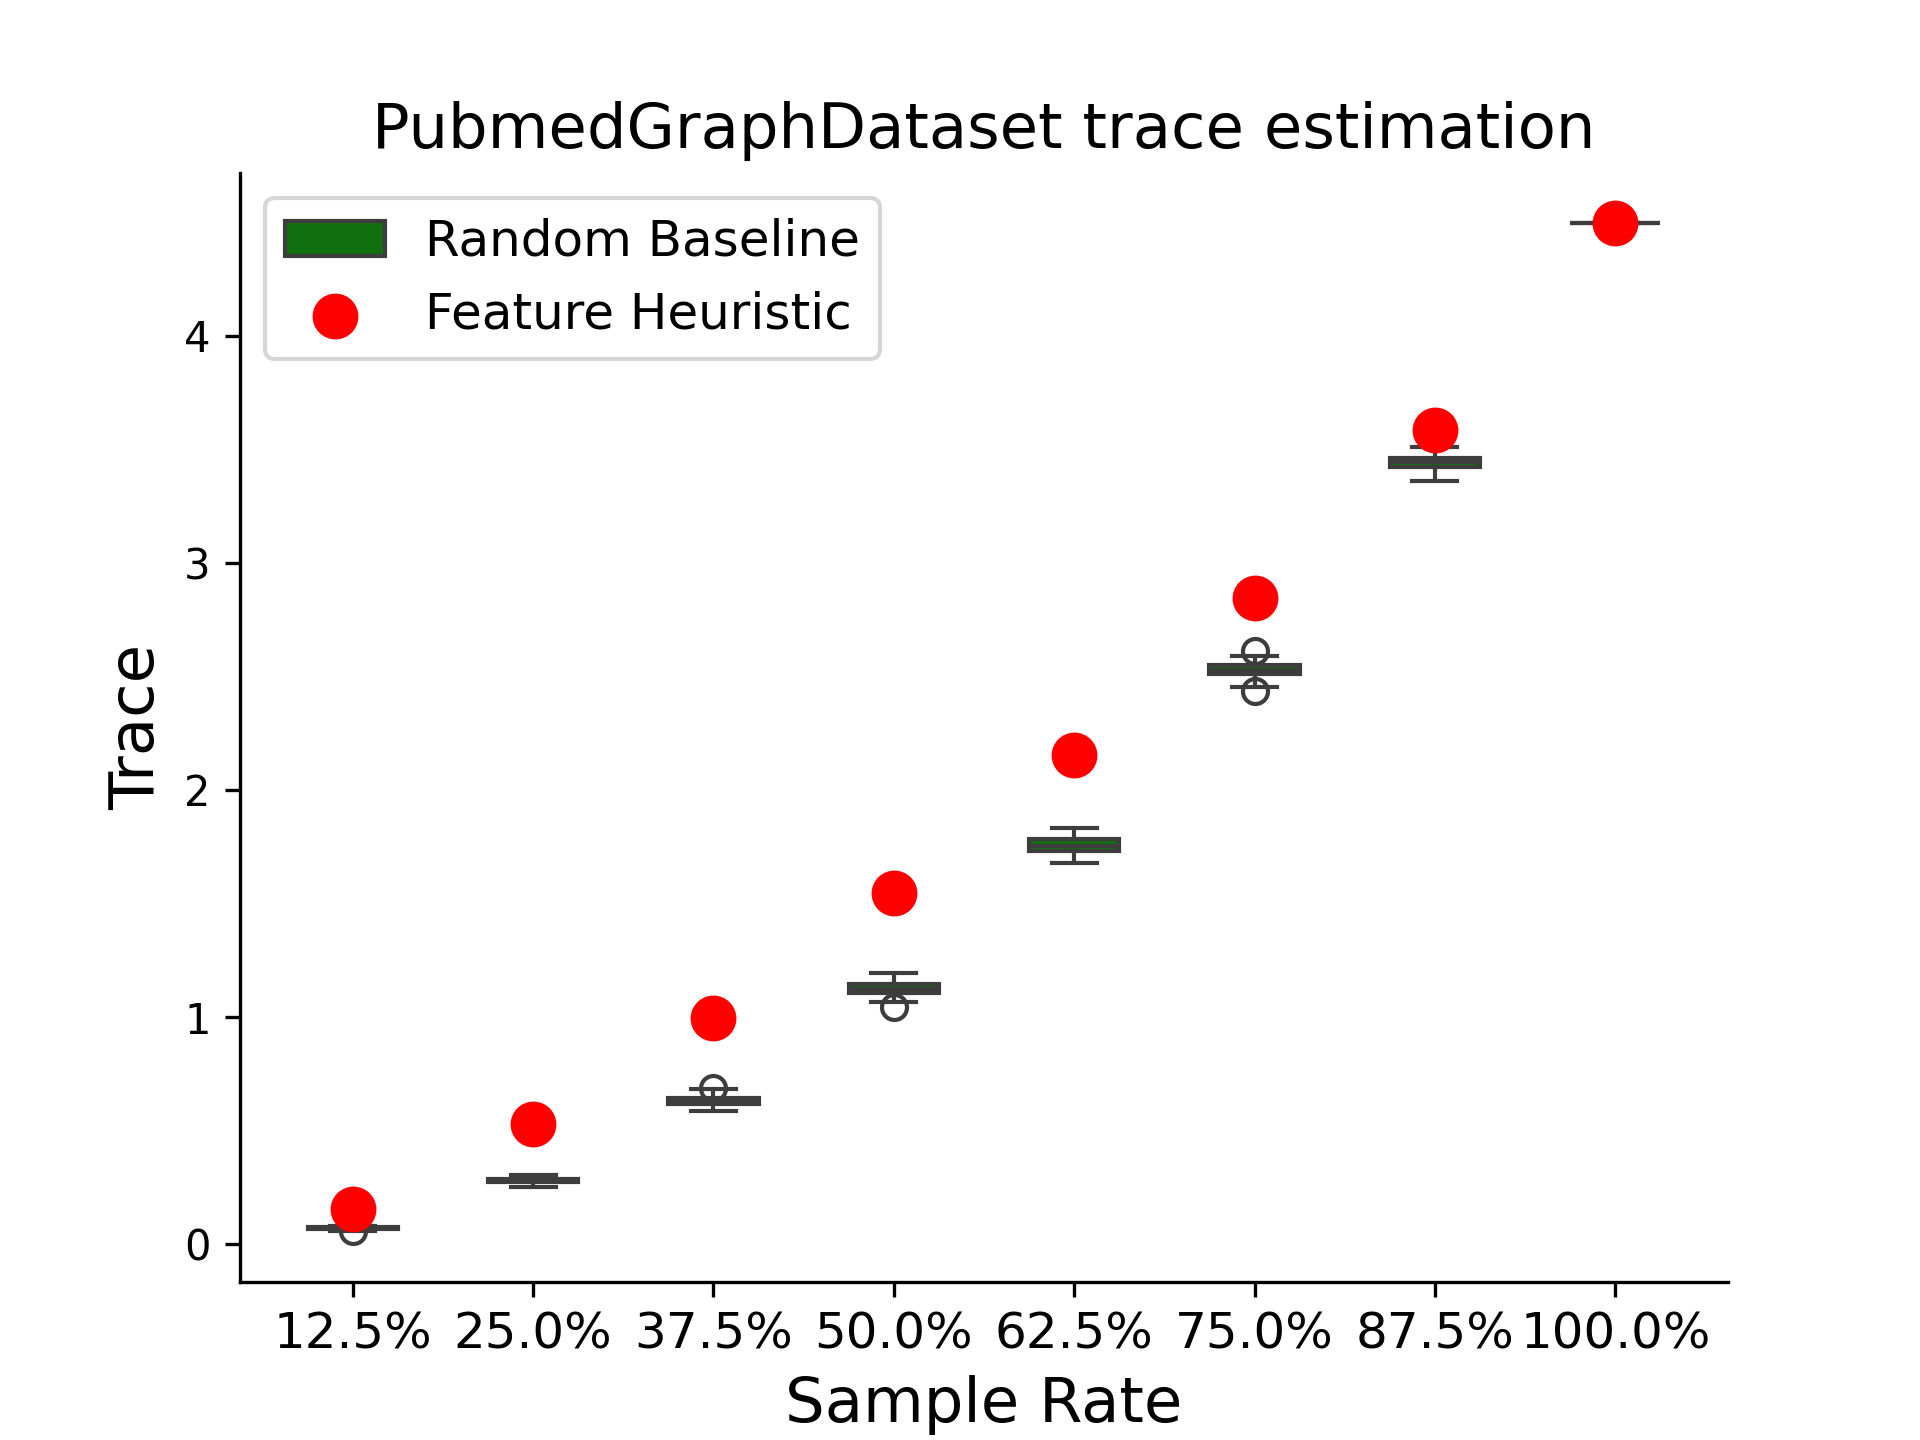
\includegraphics[width=0.32\textwidth]{img/trace_revised/PubmedGraphDataset_trace_boxplot.png}
\caption{This figure illustrates how does the trace of Laplacian change with respect to sample rate. Boxplots in the figure indicate the result obtained from random baselines in 50 runs, and the red dots are the adjusted trace of subgraphs generated by our sampling heuristic. Trace obtained by our result is almost always better than the average of random baselines except for Cora at 75\%. The adjusted trace is calculated by dividing the number of nodes in the subgraphs.}
\label{fig:trace}
\end{figure*}

\noindent \textbf{Expressivity.} While GNNs achieve remarkable performance in many graph machine learning tasks, they have fundamental limitations associated with their expressive power \cite{xu2018how,chen2019equivalence}. In GSP problems specifically, the expressivity of a GNN is constrained by the expressivity of the graph convolution, which in turn is constrained by the rank of the graph shift operator \cite{ruiz2024spectral}. This is demonstrated in the following proposition.

\begin{proposition}[Expressivity of Graph Convolution]
Let $G$ be an $n$-node symmetric graph with rank-$r$ graph shift operator $\mathbf{S}$, $r < n$, and $x \in \reals^n$ an arbitrary graph signal. Consider the graph convolution $\hat{y} = \sum_{k=0}^{K-1}h_k\mathbf{S}^kx$. Let $\ccalY \subset \reals^n$ be the subspace of signals that can be expressed as $y=\hat{y}$ for some $h_0, \ldots, h_{K-1}$. Then, $dim(\ccalY) \leq r + 1$.
\end{proposition}
\begin{proof}
   See the appendices of the extended version, available \red{\href{here}{here}}. 
\end{proof}

%\red{L: Check. James, can you check if the above proposition is true when you get a chance?}

In other words, the space of signals that can be represented with a graph convolution shrinks with the rank of the graph shift. Rank preservation is hence an important consideration when sampling subgraphs for training GNNs.